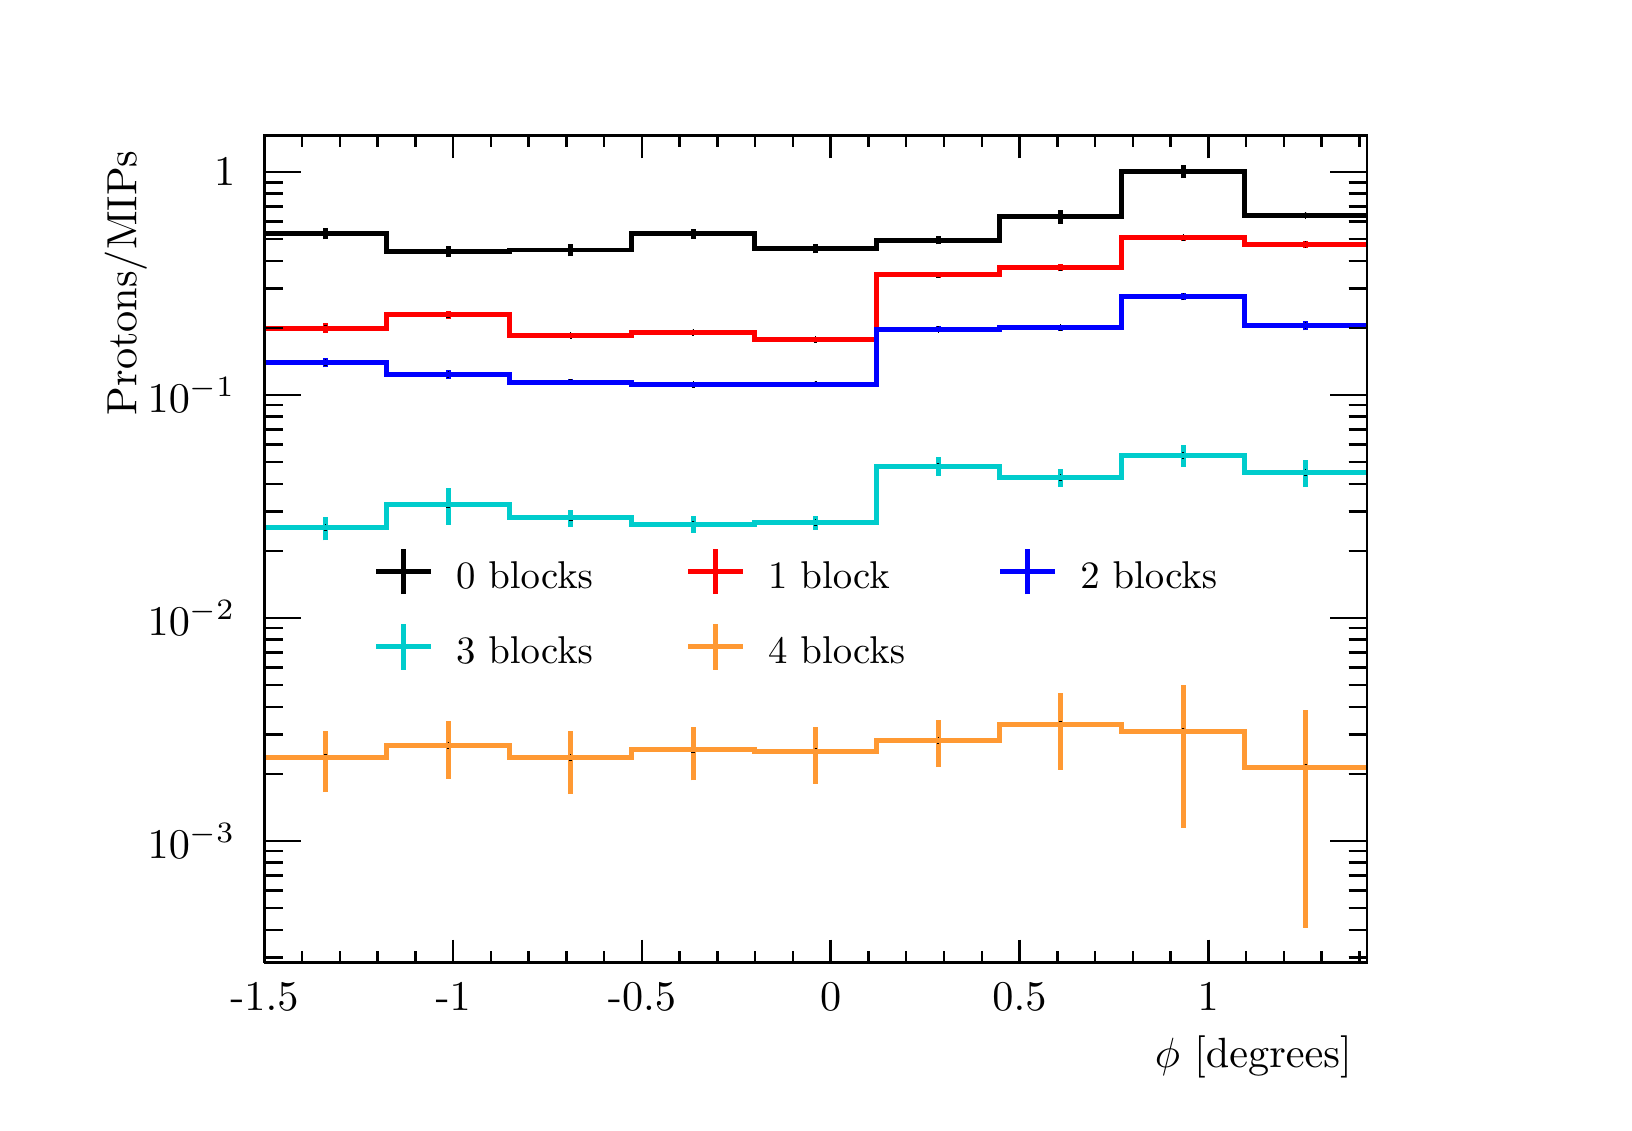
\begin{tikzpicture}
\pgfdeclareplotmark{cross} {
\pgfpathmoveto{\pgfpoint{-0.3\pgfplotmarksize}{\pgfplotmarksize}}
\pgfpathlineto{\pgfpoint{+0.3\pgfplotmarksize}{\pgfplotmarksize}}
\pgfpathlineto{\pgfpoint{+0.3\pgfplotmarksize}{0.3\pgfplotmarksize}}
\pgfpathlineto{\pgfpoint{+1\pgfplotmarksize}{0.3\pgfplotmarksize}}
\pgfpathlineto{\pgfpoint{+1\pgfplotmarksize}{-0.3\pgfplotmarksize}}
\pgfpathlineto{\pgfpoint{+0.3\pgfplotmarksize}{-0.3\pgfplotmarksize}}
\pgfpathlineto{\pgfpoint{+0.3\pgfplotmarksize}{-1.\pgfplotmarksize}}
\pgfpathlineto{\pgfpoint{-0.3\pgfplotmarksize}{-1.\pgfplotmarksize}}
\pgfpathlineto{\pgfpoint{-0.3\pgfplotmarksize}{-0.3\pgfplotmarksize}}
\pgfpathlineto{\pgfpoint{-1.\pgfplotmarksize}{-0.3\pgfplotmarksize}}
\pgfpathlineto{\pgfpoint{-1.\pgfplotmarksize}{0.3\pgfplotmarksize}}
\pgfpathlineto{\pgfpoint{-0.3\pgfplotmarksize}{0.3\pgfplotmarksize}}
\pgfpathclose
\pgfusepathqstroke
}
\pgfdeclareplotmark{cross*} {
\pgfpathmoveto{\pgfpoint{-0.3\pgfplotmarksize}{\pgfplotmarksize}}
\pgfpathlineto{\pgfpoint{+0.3\pgfplotmarksize}{\pgfplotmarksize}}
\pgfpathlineto{\pgfpoint{+0.3\pgfplotmarksize}{0.3\pgfplotmarksize}}
\pgfpathlineto{\pgfpoint{+1\pgfplotmarksize}{0.3\pgfplotmarksize}}
\pgfpathlineto{\pgfpoint{+1\pgfplotmarksize}{-0.3\pgfplotmarksize}}
\pgfpathlineto{\pgfpoint{+0.3\pgfplotmarksize}{-0.3\pgfplotmarksize}}
\pgfpathlineto{\pgfpoint{+0.3\pgfplotmarksize}{-1.\pgfplotmarksize}}
\pgfpathlineto{\pgfpoint{-0.3\pgfplotmarksize}{-1.\pgfplotmarksize}}
\pgfpathlineto{\pgfpoint{-0.3\pgfplotmarksize}{-0.3\pgfplotmarksize}}
\pgfpathlineto{\pgfpoint{-1.\pgfplotmarksize}{-0.3\pgfplotmarksize}}
\pgfpathlineto{\pgfpoint{-1.\pgfplotmarksize}{0.3\pgfplotmarksize}}
\pgfpathlineto{\pgfpoint{-0.3\pgfplotmarksize}{0.3\pgfplotmarksize}}
\pgfpathclose
\pgfusepathqfillstroke
}
\pgfdeclareplotmark{newstar} {
\pgfpathmoveto{\pgfqpoint{0pt}{\pgfplotmarksize}}
\pgfpathlineto{\pgfqpointpolar{44}{0.5\pgfplotmarksize}}
\pgfpathlineto{\pgfqpointpolar{18}{\pgfplotmarksize}}
\pgfpathlineto{\pgfqpointpolar{-20}{0.5\pgfplotmarksize}}
\pgfpathlineto{\pgfqpointpolar{-54}{\pgfplotmarksize}}
\pgfpathlineto{\pgfqpointpolar{-90}{0.5\pgfplotmarksize}}
\pgfpathlineto{\pgfqpointpolar{234}{\pgfplotmarksize}}
\pgfpathlineto{\pgfqpointpolar{198}{0.5\pgfplotmarksize}}
\pgfpathlineto{\pgfqpointpolar{162}{\pgfplotmarksize}}
\pgfpathlineto{\pgfqpointpolar{134}{0.5\pgfplotmarksize}}
\pgfpathclose
\pgfusepathqstroke
}
\pgfdeclareplotmark{newstar*} {
\pgfpathmoveto{\pgfqpoint{0pt}{\pgfplotmarksize}}
\pgfpathlineto{\pgfqpointpolar{44}{0.5\pgfplotmarksize}}
\pgfpathlineto{\pgfqpointpolar{18}{\pgfplotmarksize}}
\pgfpathlineto{\pgfqpointpolar{-20}{0.5\pgfplotmarksize}}
\pgfpathlineto{\pgfqpointpolar{-54}{\pgfplotmarksize}}
\pgfpathlineto{\pgfqpointpolar{-90}{0.5\pgfplotmarksize}}
\pgfpathlineto{\pgfqpointpolar{234}{\pgfplotmarksize}}
\pgfpathlineto{\pgfqpointpolar{198}{0.5\pgfplotmarksize}}
\pgfpathlineto{\pgfqpointpolar{162}{\pgfplotmarksize}}
\pgfpathlineto{\pgfqpointpolar{134}{0.5\pgfplotmarksize}}
\pgfpathclose
\pgfusepathqfillstroke
}
\definecolor{c}{rgb}{1,1,1};
\draw [color=c, fill=c] (0,0) rectangle (20,13.639);
\draw [color=c, fill=c] (3,1.77307) rectangle (17,12.2751);
\definecolor{c}{rgb}{0,0,0};
\draw [c,line width=0.9] (3,1.77307) -- (3,12.2751) -- (17,12.2751) -- (17,1.77307) -- (3,1.77307);
\definecolor{c}{rgb}{1,1,1};
\draw [color=c, fill=c] (3,1.77307) rectangle (17,12.2751);
\definecolor{c}{rgb}{0,0,0};
\draw [c,line width=0.9] (3,1.77307) -- (3,12.2751) -- (17,12.2751) -- (17,1.77307) -- (3,1.77307);
\draw [c,line width=0.9] (3,1.77307) -- (4.55556,1.77307) -- (4.55556,1.77307) -- (6.11111,1.77307) -- (6.11111,1.77307) -- (7.66667,1.77307) -- (7.66667,1.77307) -- (9.22222,1.77307) -- (9.22222,1.77307) -- (10.7778,1.77307) -- (10.7778,1.77307) --
 (12.3333,1.77307) -- (12.3333,1.77307) -- (13.8889,1.77307) -- (13.8889,1.77307) -- (15.4444,1.77307) -- (15.4444,1.77307) -- (17,1.77307);
\draw [c,line width=0.9] (3,1.77307) -- (17,1.77307);
\draw [c,line width=0.9] (3,2.05948) -- (3,1.77307);
\draw [c,line width=0.9] (3.47945,1.91628) -- (3.47945,1.77307);
\draw [c,line width=0.9] (3.9589,1.91628) -- (3.9589,1.77307);
\draw [c,line width=0.9] (4.43836,1.91628) -- (4.43836,1.77307);
\draw [c,line width=0.9] (4.91781,1.91628) -- (4.91781,1.77307);
\draw [c,line width=0.9] (5.39726,2.05948) -- (5.39726,1.77307);
\draw [c,line width=0.9] (5.87671,1.91628) -- (5.87671,1.77307);
\draw [c,line width=0.9] (6.35616,1.91628) -- (6.35616,1.77307);
\draw [c,line width=0.9] (6.83562,1.91628) -- (6.83562,1.77307);
\draw [c,line width=0.9] (7.31507,1.91628) -- (7.31507,1.77307);
\draw [c,line width=0.9] (7.79452,2.05948) -- (7.79452,1.77307);
\draw [c,line width=0.9] (8.27397,1.91628) -- (8.27397,1.77307);
\draw [c,line width=0.9] (8.75342,1.91628) -- (8.75342,1.77307);
\draw [c,line width=0.9] (9.23288,1.91628) -- (9.23288,1.77307);
\draw [c,line width=0.9] (9.71233,1.91628) -- (9.71233,1.77307);
\draw [c,line width=0.9] (10.1918,2.05948) -- (10.1918,1.77307);
\draw [c,line width=0.9] (10.6712,1.91628) -- (10.6712,1.77307);
\draw [c,line width=0.9] (11.1507,1.91628) -- (11.1507,1.77307);
\draw [c,line width=0.9] (11.6301,1.91628) -- (11.6301,1.77307);
\draw [c,line width=0.9] (12.1096,1.91628) -- (12.1096,1.77307);
\draw [c,line width=0.9] (12.589,2.05948) -- (12.589,1.77307);
\draw [c,line width=0.9] (13.0685,1.91628) -- (13.0685,1.77307);
\draw [c,line width=0.9] (13.5479,1.91628) -- (13.5479,1.77307);
\draw [c,line width=0.9] (14.0274,1.91628) -- (14.0274,1.77307);
\draw [c,line width=0.9] (14.5068,1.91628) -- (14.5068,1.77307);
\draw [c,line width=0.9] (14.9863,2.05948) -- (14.9863,1.77307);
\draw [c,line width=0.9] (14.9863,2.05948) -- (14.9863,1.77307);
\draw [c,line width=0.9] (15.4658,1.91628) -- (15.4658,1.77307);
\draw [c,line width=0.9] (15.9452,1.91628) -- (15.9452,1.77307);
\draw [c,line width=0.9] (16.4247,1.91628) -- (16.4247,1.77307);
\draw [c,line width=0.9] (16.9041,1.91628) -- (16.9041,1.77307);
\draw [anchor=base] (3,1.15931) node[scale=1.52731, color=c, rotate=0]{-1.5};
\draw [anchor=base] (5.39726,1.15931) node[scale=1.52731, color=c, rotate=0]{-1};
\draw [anchor=base] (7.79452,1.15931) node[scale=1.52731, color=c, rotate=0]{-0.5};
\draw [anchor=base] (10.1918,1.15931) node[scale=1.52731, color=c, rotate=0]{0};
\draw [anchor=base] (12.589,1.15931) node[scale=1.52731, color=c, rotate=0]{0.5};
\draw [anchor=base] (14.9863,1.15931) node[scale=1.52731, color=c, rotate=0]{1};
\draw [anchor= east] (17,0.572837) node[scale=1.52731, color=c, rotate=0]{$\phi$ [degrees] };
\draw [c,line width=0.9] (3,12.2751) -- (17,12.2751);
\draw [c,line width=0.9] (3,11.9887) -- (3,12.2751);
\draw [c,line width=0.9] (3.47945,12.1319) -- (3.47945,12.2751);
\draw [c,line width=0.9] (3.9589,12.1319) -- (3.9589,12.2751);
\draw [c,line width=0.9] (4.43836,12.1319) -- (4.43836,12.2751);
\draw [c,line width=0.9] (4.91781,12.1319) -- (4.91781,12.2751);
\draw [c,line width=0.9] (5.39726,11.9887) -- (5.39726,12.2751);
\draw [c,line width=0.9] (5.87671,12.1319) -- (5.87671,12.2751);
\draw [c,line width=0.9] (6.35616,12.1319) -- (6.35616,12.2751);
\draw [c,line width=0.9] (6.83562,12.1319) -- (6.83562,12.2751);
\draw [c,line width=0.9] (7.31507,12.1319) -- (7.31507,12.2751);
\draw [c,line width=0.9] (7.79452,11.9887) -- (7.79452,12.2751);
\draw [c,line width=0.9] (8.27397,12.1319) -- (8.27397,12.2751);
\draw [c,line width=0.9] (8.75342,12.1319) -- (8.75342,12.2751);
\draw [c,line width=0.9] (9.23288,12.1319) -- (9.23288,12.2751);
\draw [c,line width=0.9] (9.71233,12.1319) -- (9.71233,12.2751);
\draw [c,line width=0.9] (10.1918,11.9887) -- (10.1918,12.2751);
\draw [c,line width=0.9] (10.6712,12.1319) -- (10.6712,12.2751);
\draw [c,line width=0.9] (11.1507,12.1319) -- (11.1507,12.2751);
\draw [c,line width=0.9] (11.6301,12.1319) -- (11.6301,12.2751);
\draw [c,line width=0.9] (12.1096,12.1319) -- (12.1096,12.2751);
\draw [c,line width=0.9] (12.589,11.9887) -- (12.589,12.2751);
\draw [c,line width=0.9] (13.0685,12.1319) -- (13.0685,12.2751);
\draw [c,line width=0.9] (13.5479,12.1319) -- (13.5479,12.2751);
\draw [c,line width=0.9] (14.0274,12.1319) -- (14.0274,12.2751);
\draw [c,line width=0.9] (14.5068,12.1319) -- (14.5068,12.2751);
\draw [c,line width=0.9] (14.9863,11.9887) -- (14.9863,12.2751);
\draw [c,line width=0.9] (14.9863,11.9887) -- (14.9863,12.2751);
\draw [c,line width=0.9] (15.4658,12.1319) -- (15.4658,12.2751);
\draw [c,line width=0.9] (15.9452,12.1319) -- (15.9452,12.2751);
\draw [c,line width=0.9] (16.4247,12.1319) -- (16.4247,12.2751);
\draw [c,line width=0.9] (16.9041,12.1319) -- (16.9041,12.2751);
\draw [c,line width=0.9] (3,1.77307) -- (3,12.2751);
\draw [c,line width=0.9] (3.231,1.83556) -- (3,1.83556);
\draw [c,line width=0.9] (3.231,2.18938) -- (3,2.18938);
\draw [c,line width=0.9] (3.231,2.46382) -- (3,2.46382);
\draw [c,line width=0.9] (3.231,2.68806) -- (3,2.68806);
\draw [c,line width=0.9] (3.231,2.87766) -- (3,2.87766);
\draw [c,line width=0.9] (3.231,3.04189) -- (3,3.04189);
\draw [c,line width=0.9] (3.231,3.18675) -- (3,3.18675);
\draw [c,line width=0.9] (3.462,3.31633) -- (3,3.31633);
\draw [anchor= east] (2.82,3.31633) node[scale=1.52731, color=c, rotate=0]{$10^{-3}$};
\draw [c,line width=0.9] (3.231,4.16884) -- (3,4.16884);
\draw [c,line width=0.9] (3.231,4.66753) -- (3,4.66753);
\draw [c,line width=0.9] (3.231,5.02135) -- (3,5.02135);
\draw [c,line width=0.9] (3.231,5.2958) -- (3,5.2958);
\draw [c,line width=0.9] (3.231,5.52004) -- (3,5.52004);
\draw [c,line width=0.9] (3.231,5.70963) -- (3,5.70963);
\draw [c,line width=0.9] (3.231,5.87386) -- (3,5.87386);
\draw [c,line width=0.9] (3.231,6.01872) -- (3,6.01872);
\draw [c,line width=0.9] (3.462,6.1483) -- (3,6.1483);
\draw [anchor= east] (2.82,6.1483) node[scale=1.52731, color=c, rotate=0]{$10^{-2}$};
\draw [c,line width=0.9] (3.231,7.00081) -- (3,7.00081);
\draw [c,line width=0.9] (3.231,7.4995) -- (3,7.4995);
\draw [c,line width=0.9] (3.231,7.85332) -- (3,7.85332);
\draw [c,line width=0.9] (3.231,8.12777) -- (3,8.12777);
\draw [c,line width=0.9] (3.231,8.35201) -- (3,8.35201);
\draw [c,line width=0.9] (3.231,8.5416) -- (3,8.5416);
\draw [c,line width=0.9] (3.231,8.70583) -- (3,8.70583);
\draw [c,line width=0.9] (3.231,8.85069) -- (3,8.85069);
\draw [c,line width=0.9] (3.462,8.98028) -- (3,8.98028);
\draw [anchor= east] (2.82,8.98028) node[scale=1.52731, color=c, rotate=0]{$10^{-1}$};
\draw [c,line width=0.9] (3.231,9.83278) -- (3,9.83278);
\draw [c,line width=0.9] (3.231,10.3315) -- (3,10.3315);
\draw [c,line width=0.9] (3.231,10.6853) -- (3,10.6853);
\draw [c,line width=0.9] (3.231,10.9597) -- (3,10.9597);
\draw [c,line width=0.9] (3.231,11.184) -- (3,11.184);
\draw [c,line width=0.9] (3.231,11.3736) -- (3,11.3736);
\draw [c,line width=0.9] (3.231,11.5378) -- (3,11.5378);
\draw [c,line width=0.9] (3.231,11.6827) -- (3,11.6827);
\draw [c,line width=0.9] (3.462,11.8122) -- (3,11.8122);
\draw [anchor= east] (2.82,11.8122) node[scale=1.52731, color=c, rotate=0]{1};
\draw [anchor= east] (1.24,12.2751) node[scale=1.52731, color=c, rotate=90]{ Protons/MIPs};
\draw [c,line width=0.9] (17,1.77307) -- (17,12.2751);
\draw [c,line width=0.9] (16.769,1.83556) -- (17,1.83556);
\draw [c,line width=0.9] (16.769,2.18938) -- (17,2.18938);
\draw [c,line width=0.9] (16.769,2.46382) -- (17,2.46382);
\draw [c,line width=0.9] (16.769,2.68806) -- (17,2.68806);
\draw [c,line width=0.9] (16.769,2.87766) -- (17,2.87766);
\draw [c,line width=0.9] (16.769,3.04189) -- (17,3.04189);
\draw [c,line width=0.9] (16.769,3.18675) -- (17,3.18675);
\draw [c,line width=0.9] (16.538,3.31633) -- (17,3.31633);
\draw [c,line width=0.9] (16.769,4.16884) -- (17,4.16884);
\draw [c,line width=0.9] (16.769,4.66753) -- (17,4.66753);
\draw [c,line width=0.9] (16.769,5.02135) -- (17,5.02135);
\draw [c,line width=0.9] (16.769,5.2958) -- (17,5.2958);
\draw [c,line width=0.9] (16.769,5.52004) -- (17,5.52004);
\draw [c,line width=0.9] (16.769,5.70963) -- (17,5.70963);
\draw [c,line width=0.9] (16.769,5.87386) -- (17,5.87386);
\draw [c,line width=0.9] (16.769,6.01872) -- (17,6.01872);
\draw [c,line width=0.9] (16.538,6.1483) -- (17,6.1483);
\draw [c,line width=0.9] (16.769,7.00081) -- (17,7.00081);
\draw [c,line width=0.9] (16.769,7.4995) -- (17,7.4995);
\draw [c,line width=0.9] (16.769,7.85332) -- (17,7.85332);
\draw [c,line width=0.9] (16.769,8.12777) -- (17,8.12777);
\draw [c,line width=0.9] (16.769,8.35201) -- (17,8.35201);
\draw [c,line width=0.9] (16.769,8.5416) -- (17,8.5416);
\draw [c,line width=0.9] (16.769,8.70583) -- (17,8.70583);
\draw [c,line width=0.9] (16.769,8.85069) -- (17,8.85069);
\draw [c,line width=0.9] (16.538,8.98028) -- (17,8.98028);
\draw [c,line width=0.9] (16.769,9.83278) -- (17,9.83278);
\draw [c,line width=0.9] (16.769,10.3315) -- (17,10.3315);
\draw [c,line width=0.9] (16.769,10.6853) -- (17,10.6853);
\draw [c,line width=0.9] (16.769,10.9597) -- (17,10.9597);
\draw [c,line width=0.9] (16.769,11.184) -- (17,11.184);
\draw [c,line width=0.9] (16.769,11.3736) -- (17,11.3736);
\draw [c,line width=0.9] (16.769,11.5378) -- (17,11.5378);
\draw [c,line width=0.9] (16.769,11.6827) -- (17,11.6827);
\draw [c,line width=0.9] (16.538,11.8122) -- (17,11.8122);
\draw [c,line width=1.8] (3.77778,10.9579) -- (3.77778,11.029);
\draw [c,line width=1.8] (3.77778,11.029) -- (3.77778,11.0961);
\foreach \P in {(3.77778,11.029)}{\draw[mark options={color=c,fill=c},mark size=2.402402pt, line width=0.000000pt, mark=*,mark size=1pt] plot coordinates {\P};}
\draw [c,line width=1.8] (5.33333,10.7306) -- (5.33333,10.8035);
\draw [c,line width=1.8] (5.33333,10.8035) -- (5.33333,10.8724);
\foreach \P in {(5.33333,10.8035)}{\draw[mark options={color=c,fill=c},mark size=2.402402pt, line width=0.000000pt, mark=*,mark size=1pt] plot coordinates {\P};}
\draw [c,line width=1.8] (6.88889,10.7423) -- (6.88889,10.8223);
\draw [c,line width=1.8] (6.88889,10.8223) -- (6.88889,10.8974);
\foreach \P in {(6.88889,10.8223)}{\draw[mark options={color=c,fill=c},mark size=2.402402pt, line width=0.000000pt, mark=*,mark size=1pt] plot coordinates {\P};}
\draw [c,line width=1.8] (8.44444,10.9682) -- (8.44444,11.0313);
\draw [c,line width=1.8] (8.44444,11.0313) -- (8.44444,11.0913);
\foreach \P in {(8.44444,11.0313)}{\draw[mark options={color=c,fill=c},mark size=2.402402pt, line width=0.000000pt, mark=*,mark size=1pt] plot coordinates {\P};}
\draw [c,line width=1.8] (10,10.7787) -- (10,10.8393);
\draw [c,line width=1.8] (10,10.8393) -- (10,10.8971);
\foreach \P in {(10,10.8393)}{\draw[mark options={color=c,fill=c},mark size=2.402402pt, line width=0.000000pt, mark=*,mark size=1pt] plot coordinates {\P};}
\draw [c,line width=1.8] (11.5556,10.8944) -- (11.5556,10.9462);
\draw [c,line width=1.8] (11.5556,10.9462) -- (11.5556,10.9958);
\foreach \P in {(11.5556,10.9462)}{\draw[mark options={color=c,fill=c},mark size=2.402402pt, line width=0.000000pt, mark=*,mark size=1pt] plot coordinates {\P};}
\draw [c,line width=1.8] (13.1111,11.1572) -- (13.1111,11.2435);
\draw [c,line width=1.8] (13.1111,11.2435) -- (13.1111,11.3241);
\foreach \P in {(13.1111,11.2435)}{\draw[mark options={color=c,fill=c},mark size=2.402402pt, line width=0.000000pt, mark=*,mark size=1pt] plot coordinates {\P};}
\draw [c,line width=1.8] (14.6667,11.7352) -- (14.6667,11.8234);
\draw [c,line width=1.8] (14.6667,11.8234) -- (14.6667,11.9056);
\foreach \P in {(14.6667,11.8234)}{\draw[mark options={color=c,fill=c},mark size=2.402402pt, line width=0.000000pt, mark=*,mark size=1pt] plot coordinates {\P};}
\draw [c,line width=1.8] (16.2222,11.2378) -- (16.2222,11.2633);
\draw [c,line width=1.8] (16.2222,11.2633) -- (16.2222,11.2883);
\foreach \P in {(16.2222,11.2633)}{\draw[mark options={color=c,fill=c},mark size=2.402402pt, line width=0.000000pt, mark=*,mark size=1pt] plot coordinates {\P};}
\draw [c,line width=1.8] (3,11.029) -- (4.55556,11.029) -- (4.55556,10.8035) -- (6.11111,10.8035) -- (6.11111,10.8223) -- (7.66667,10.8223) -- (7.66667,11.0313) -- (9.22222,11.0313) -- (9.22222,10.8393) -- (10.7778,10.8393) -- (10.7778,10.9462) --
 (12.3333,10.9462) -- (12.3333,11.2435) -- (13.8889,11.2435) -- (13.8889,11.8234) -- (15.4444,11.8234) -- (15.4444,11.2633) -- (17,11.2633);
\definecolor{c}{rgb}{1,0,0};
\draw [c,line width=1.8] (3.77778,9.77115) -- (3.77778,9.8315);
\draw [c,line width=1.8] (3.77778,9.8315) -- (3.77778,9.88903);
\definecolor{c}{rgb}{0,0,0};
\foreach \P in {(3.77778,9.8315)}{\draw[mark options={color=c,fill=c},mark size=2.402402pt, line width=0.000000pt, mark=*,mark size=1pt] plot coordinates {\P};}
\definecolor{c}{rgb}{1,0,0};
\draw [c,line width=1.8] (5.33333,9.94885) -- (5.33333,9.99961);
\draw [c,line width=1.8] (5.33333,9.99961) -- (5.33333,10.0484);
\definecolor{c}{rgb}{0,0,0};
\foreach \P in {(5.33333,9.99961)}{\draw[mark options={color=c,fill=c},mark size=2.402402pt, line width=0.000000pt, mark=*,mark size=1pt] plot coordinates {\P};}
\definecolor{c}{rgb}{1,0,0};
\draw [c,line width=1.8] (6.88889,9.70171) -- (6.88889,9.73747);
\draw [c,line width=1.8] (6.88889,9.73747) -- (6.88889,9.77221);
\definecolor{c}{rgb}{0,0,0};
\foreach \P in {(6.88889,9.73747)}{\draw[mark options={color=c,fill=c},mark size=2.402402pt, line width=0.000000pt, mark=*,mark size=1pt] plot coordinates {\P};}
\definecolor{c}{rgb}{1,0,0};
\draw [c,line width=1.8] (8.44444,9.73732) -- (8.44444,9.7754);
\draw [c,line width=1.8] (8.44444,9.7754) -- (8.44444,9.81234);
\definecolor{c}{rgb}{0,0,0};
\foreach \P in {(8.44444,9.7754)}{\draw[mark options={color=c,fill=c},mark size=2.402402pt, line width=0.000000pt, mark=*,mark size=1pt] plot coordinates {\P};}
\definecolor{c}{rgb}{1,0,0};
\draw [c,line width=1.8] (10,9.65076) -- (10,9.68293);
\draw [c,line width=1.8] (10,9.68293) -- (10,9.71428);
\definecolor{c}{rgb}{0,0,0};
\foreach \P in {(10,9.68293)}{\draw[mark options={color=c,fill=c},mark size=2.402402pt, line width=0.000000pt, mark=*,mark size=1pt] plot coordinates {\P};}
\definecolor{c}{rgb}{1,0,0};
\draw [c,line width=1.8] (11.5556,10.4709) -- (11.5556,10.5057);
\draw [c,line width=1.8] (11.5556,10.5057) -- (11.5556,10.5395);
\definecolor{c}{rgb}{0,0,0};
\foreach \P in {(11.5556,10.5057)}{\draw[mark options={color=c,fill=c},mark size=2.402402pt, line width=0.000000pt, mark=*,mark size=1pt] plot coordinates {\P};}
\definecolor{c}{rgb}{1,0,0};
\draw [c,line width=1.8] (13.1111,10.5494) -- (13.1111,10.5966);
\draw [c,line width=1.8] (13.1111,10.5966) -- (13.1111,10.642);
\definecolor{c}{rgb}{0,0,0};
\foreach \P in {(13.1111,10.5966)}{\draw[mark options={color=c,fill=c},mark size=2.402402pt, line width=0.000000pt, mark=*,mark size=1pt] plot coordinates {\P};}
\definecolor{c}{rgb}{1,0,0};
\draw [c,line width=1.8] (14.6667,10.9421) -- (14.6667,10.9797);
\draw [c,line width=1.8] (14.6667,10.9797) -- (14.6667,11.0162);
\definecolor{c}{rgb}{0,0,0};
\foreach \P in {(14.6667,10.9797)}{\draw[mark options={color=c,fill=c},mark size=2.402402pt, line width=0.000000pt, mark=*,mark size=1pt] plot coordinates {\P};}
\definecolor{c}{rgb}{1,0,0};
\draw [c,line width=1.8] (16.2222,10.8515) -- (16.2222,10.8949);
\draw [c,line width=1.8] (16.2222,10.8949) -- (16.2222,10.9368);
\definecolor{c}{rgb}{0,0,0};
\foreach \P in {(16.2222,10.8949)}{\draw[mark options={color=c,fill=c},mark size=2.402402pt, line width=0.000000pt, mark=*,mark size=1pt] plot coordinates {\P};}
\definecolor{c}{rgb}{1,0,0};
\draw [c,line width=1.8] (3,9.8315) -- (4.55556,9.8315) -- (4.55556,9.99961) -- (6.11111,9.99961) -- (6.11111,9.73747) -- (7.66667,9.73747) -- (7.66667,9.7754) -- (9.22222,9.7754) -- (9.22222,9.68293) -- (10.7778,9.68293) -- (10.7778,10.5057) --
 (12.3333,10.5057) -- (12.3333,10.5966) -- (13.8889,10.5966) -- (13.8889,10.9797) -- (15.4444,10.9797) -- (15.4444,10.8949) -- (17,10.8949);
\definecolor{c}{rgb}{0,0,1};
\draw [c,line width=1.8] (3.77778,9.33055) -- (3.77778,9.391);
\draw [c,line width=1.8] (3.77778,9.391) -- (3.77778,9.44862);
\definecolor{c}{rgb}{0,0,0};
\foreach \P in {(3.77778,9.391)}{\draw[mark options={color=c,fill=c},mark size=2.402402pt, line width=0.000000pt, mark=*,mark size=1pt] plot coordinates {\P};}
\definecolor{c}{rgb}{0,0,1};
\draw [c,line width=1.8] (5.33333,9.18882) -- (5.33333,9.24206);
\draw [c,line width=1.8] (5.33333,9.24206) -- (5.33333,9.29309);
\definecolor{c}{rgb}{0,0,0};
\foreach \P in {(5.33333,9.24206)}{\draw[mark options={color=c,fill=c},mark size=2.402402pt, line width=0.000000pt, mark=*,mark size=1pt] plot coordinates {\P};}
\definecolor{c}{rgb}{0,0,1};
\draw [c,line width=1.8] (6.88889,9.10478) -- (6.88889,9.14502);
\draw [c,line width=1.8] (6.88889,9.14502) -- (6.88889,9.18398);
\definecolor{c}{rgb}{0,0,0};
\foreach \P in {(6.88889,9.14502)}{\draw[mark options={color=c,fill=c},mark size=2.402402pt, line width=0.000000pt, mark=*,mark size=1pt] plot coordinates {\P};}
\definecolor{c}{rgb}{0,0,1};
\draw [c,line width=1.8] (8.44444,9.07774) -- (8.44444,9.1128);
\draw [c,line width=1.8] (8.44444,9.1128) -- (8.44444,9.14688);
\definecolor{c}{rgb}{0,0,0};
\foreach \P in {(8.44444,9.1128)}{\draw[mark options={color=c,fill=c},mark size=2.402402pt, line width=0.000000pt, mark=*,mark size=1pt] plot coordinates {\P};}
\definecolor{c}{rgb}{0,0,1};
\draw [c,line width=1.8] (10,9.08797) -- (10,9.11826);
\draw [c,line width=1.8] (10,9.11826) -- (10,9.14782);
\definecolor{c}{rgb}{0,0,0};
\foreach \P in {(10,9.11826)}{\draw[mark options={color=c,fill=c},mark size=2.402402pt, line width=0.000000pt, mark=*,mark size=1pt] plot coordinates {\P};}
\definecolor{c}{rgb}{0,0,1};
\draw [c,line width=1.8] (11.5556,9.77983) -- (11.5556,9.81587);
\draw [c,line width=1.8] (11.5556,9.81587) -- (11.5556,9.85088);
\definecolor{c}{rgb}{0,0,0};
\foreach \P in {(11.5556,9.81587)}{\draw[mark options={color=c,fill=c},mark size=2.402402pt, line width=0.000000pt, mark=*,mark size=1pt] plot coordinates {\P};}
\definecolor{c}{rgb}{0,0,1};
\draw [c,line width=1.8] (13.1111,9.79854) -- (13.1111,9.83698);
\draw [c,line width=1.8] (13.1111,9.83698) -- (13.1111,9.87426);
\definecolor{c}{rgb}{0,0,0};
\foreach \P in {(13.1111,9.83698)}{\draw[mark options={color=c,fill=c},mark size=2.402402pt, line width=0.000000pt, mark=*,mark size=1pt] plot coordinates {\P};}
\definecolor{c}{rgb}{0,0,1};
\draw [c,line width=1.8] (14.6667,10.1822) -- (14.6667,10.233);
\draw [c,line width=1.8] (14.6667,10.233) -- (14.6667,10.2818);
\definecolor{c}{rgb}{0,0,0};
\foreach \P in {(14.6667,10.233)}{\draw[mark options={color=c,fill=c},mark size=2.402402pt, line width=0.000000pt, mark=*,mark size=1pt] plot coordinates {\P};}
\definecolor{c}{rgb}{0,0,1};
\draw [c,line width=1.8] (16.2222,9.80138) -- (16.2222,9.86534);
\draw [c,line width=1.8] (16.2222,9.86534) -- (16.2222,9.92613);
\definecolor{c}{rgb}{0,0,0};
\foreach \P in {(16.2222,9.86534)}{\draw[mark options={color=c,fill=c},mark size=2.402402pt, line width=0.000000pt, mark=*,mark size=1pt] plot coordinates {\P};}
\definecolor{c}{rgb}{0,0,1};
\draw [c,line width=1.8] (3,9.391) -- (4.55556,9.391) -- (4.55556,9.24206) -- (6.11111,9.24206) -- (6.11111,9.14502) -- (7.66667,9.14502) -- (7.66667,9.1128) -- (9.22222,9.1128) -- (9.22222,9.11826) -- (10.7778,9.11826) -- (10.7778,9.81587) --
 (12.3333,9.81587) -- (12.3333,9.83698) -- (13.8889,9.83698) -- (13.8889,10.233) -- (15.4444,10.233) -- (15.4444,9.86534) -- (17,9.86534);
\definecolor{c}{rgb}{0,0.8,0.8};
\draw [c,line width=1.8] (3.77778,7.1338) -- (3.77778,7.29514);
\draw [c,line width=1.8] (3.77778,7.29514) -- (3.77778,7.43775);
\definecolor{c}{rgb}{0,0,0};
\foreach \P in {(3.77778,7.29514)}{\draw[mark options={color=c,fill=c},mark size=2.402402pt, line width=0.000000pt, mark=*,mark size=1pt] plot coordinates {\P};}
\definecolor{c}{rgb}{0,0.8,0.8};
\draw [c,line width=1.8] (5.33333,7.33297) -- (5.33333,7.58594);
\draw [c,line width=1.8] (5.33333,7.58594) -- (5.33333,7.79565);
\definecolor{c}{rgb}{0,0,0};
\foreach \P in {(5.33333,7.58594)}{\draw[mark options={color=c,fill=c},mark size=2.402402pt, line width=0.000000pt, mark=*,mark size=1pt] plot coordinates {\P};}
\definecolor{c}{rgb}{0,0.8,0.8};
\draw [c,line width=1.8] (6.88889,7.30754) -- (6.88889,7.4209);
\draw [c,line width=1.8] (6.88889,7.4209) -- (6.88889,7.52468);
\definecolor{c}{rgb}{0,0,0};
\foreach \P in {(6.88889,7.4209)}{\draw[mark options={color=c,fill=c},mark size=2.402402pt, line width=0.000000pt, mark=*,mark size=1pt] plot coordinates {\P};}
\definecolor{c}{rgb}{0,0.8,0.8};
\draw [c,line width=1.8] (8.44444,7.22568) -- (8.44444,7.34084);
\draw [c,line width=1.8] (8.44444,7.34084) -- (8.44444,7.44614);
\definecolor{c}{rgb}{0,0,0};
\foreach \P in {(8.44444,7.34084)}{\draw[mark options={color=c,fill=c},mark size=2.402402pt, line width=0.000000pt, mark=*,mark size=1pt] plot coordinates {\P};}
\definecolor{c}{rgb}{0,0.8,0.8};
\draw [c,line width=1.8] (10,7.2676) -- (10,7.35861);
\draw [c,line width=1.8] (10,7.35861) -- (10,7.44335);
\definecolor{c}{rgb}{0,0,0};
\foreach \P in {(10,7.35861)}{\draw[mark options={color=c,fill=c},mark size=2.402402pt, line width=0.000000pt, mark=*,mark size=1pt] plot coordinates {\P};}
\definecolor{c}{rgb}{0,0.8,0.8};
\draw [c,line width=1.8] (11.5556,7.95478) -- (11.5556,8.07808);
\draw [c,line width=1.8] (11.5556,8.07808) -- (11.5556,8.19013);
\definecolor{c}{rgb}{0,0,0};
\foreach \P in {(11.5556,8.07808)}{\draw[mark options={color=c,fill=c},mark size=2.402402pt, line width=0.000000pt, mark=*,mark size=1pt] plot coordinates {\P};}
\definecolor{c}{rgb}{0,0.8,0.8};
\draw [c,line width=1.8] (13.1111,7.81262) -- (13.1111,7.93134);
\draw [c,line width=1.8] (13.1111,7.93134) -- (13.1111,8.03961);
\definecolor{c}{rgb}{0,0,0};
\foreach \P in {(13.1111,7.93134)}{\draw[mark options={color=c,fill=c},mark size=2.402402pt, line width=0.000000pt, mark=*,mark size=1pt] plot coordinates {\P};}
\definecolor{c}{rgb}{0,0.8,0.8};
\draw [c,line width=1.8] (14.6667,8.07276) -- (14.6667,8.21503);
\draw [c,line width=1.8] (14.6667,8.21503) -- (14.6667,8.34254);
\definecolor{c}{rgb}{0,0,0};
\foreach \P in {(14.6667,8.21503)}{\draw[mark options={color=c,fill=c},mark size=2.402402pt, line width=0.000000pt, mark=*,mark size=1pt] plot coordinates {\P};}
\definecolor{c}{rgb}{0,0.8,0.8};
\draw [c,line width=1.8] (16.2222,7.81053) -- (16.2222,7.99503);
\draw [c,line width=1.8] (16.2222,7.99503) -- (16.2222,8.15543);
\definecolor{c}{rgb}{0,0,0};
\foreach \P in {(16.2222,7.99503)}{\draw[mark options={color=c,fill=c},mark size=2.402402pt, line width=0.000000pt, mark=*,mark size=1pt] plot coordinates {\P};}
\definecolor{c}{rgb}{0,0.8,0.8};
\draw [c,line width=1.8] (3,7.29514) -- (4.55556,7.29514) -- (4.55556,7.58594) -- (6.11111,7.58594) -- (6.11111,7.4209) -- (7.66667,7.4209) -- (7.66667,7.34084) -- (9.22222,7.34084) -- (9.22222,7.35861) -- (10.7778,7.35861) -- (10.7778,8.07808) --
 (12.3333,8.07808) -- (12.3333,7.93134) -- (13.8889,7.93134) -- (13.8889,8.21503) -- (15.4444,8.21503) -- (15.4444,7.99503) -- (17,7.99503);
\definecolor{c}{rgb}{1,0.6,0.2};
\draw [c,line width=1.8] (3.77778,3.93891) -- (3.77778,4.38291);
\draw [c,line width=1.8] (3.77778,4.38291) -- (3.77778,4.70845);
\definecolor{c}{rgb}{0,0,0};
\foreach \P in {(3.77778,4.38291)}{\draw[mark options={color=c,fill=c},mark size=2.402402pt, line width=0.000000pt, mark=*,mark size=1pt] plot coordinates {\P};}
\definecolor{c}{rgb}{1,0.6,0.2};
\draw [c,line width=1.8] (5.33333,4.10722) -- (5.33333,4.53088);
\draw [c,line width=1.8] (5.33333,4.53088) -- (5.33333,4.8454);
\definecolor{c}{rgb}{0,0,0};
\foreach \P in {(5.33333,4.53088)}{\draw[mark options={color=c,fill=c},mark size=2.402402pt, line width=0.000000pt, mark=*,mark size=1pt] plot coordinates {\P};}
\definecolor{c}{rgb}{1,0.6,0.2};
\draw [c,line width=1.8] (6.88889,3.91167) -- (6.88889,4.37654);
\draw [c,line width=1.8] (6.88889,4.37654) -- (6.88889,4.71309);
\definecolor{c}{rgb}{0,0,0};
\foreach \P in {(6.88889,4.37654)}{\draw[mark options={color=c,fill=c},mark size=2.402402pt, line width=0.000000pt, mark=*,mark size=1pt] plot coordinates {\P};}
\definecolor{c}{rgb}{1,0.6,0.2};
\draw [c,line width=1.8] (8.44444,4.08591) -- (8.44444,4.47386);
\draw [c,line width=1.8] (8.44444,4.47386) -- (8.44444,4.76834);
\definecolor{c}{rgb}{0,0,0};
\foreach \P in {(8.44444,4.47386)}{\draw[mark options={color=c,fill=c},mark size=2.402402pt, line width=0.000000pt, mark=*,mark size=1pt] plot coordinates {\P};}
\definecolor{c}{rgb}{1,0.6,0.2};
\draw [c,line width=1.8] (10,4.04462) -- (10,4.45721);
\draw [c,line width=1.8] (10,4.45721) -- (10,4.76562);
\definecolor{c}{rgb}{0,0,0};
\foreach \P in {(10,4.45721)}{\draw[mark options={color=c,fill=c},mark size=2.402402pt, line width=0.000000pt, mark=*,mark size=1pt] plot coordinates {\P};}
\definecolor{c}{rgb}{1,0.6,0.2};
\draw [c,line width=1.8] (11.5556,4.25568) -- (11.5556,4.59315);
\draw [c,line width=1.8] (11.5556,4.59315) -- (11.5556,4.85768);
\definecolor{c}{rgb}{0,0,0};
\foreach \P in {(11.5556,4.59315)}{\draw[mark options={color=c,fill=c},mark size=2.402402pt, line width=0.000000pt, mark=*,mark size=1pt] plot coordinates {\P};}
\definecolor{c}{rgb}{1,0.6,0.2};
\draw [c,line width=1.8] (13.1111,4.22098) -- (13.1111,4.80213);
\draw [c,line width=1.8] (13.1111,4.80213) -- (13.1111,5.1952);
\definecolor{c}{rgb}{0,0,0};
\foreach \P in {(13.1111,4.80213)}{\draw[mark options={color=c,fill=c},mark size=2.402402pt, line width=0.000000pt, mark=*,mark size=1pt] plot coordinates {\P};}
\definecolor{c}{rgb}{1,0.6,0.2};
\draw [c,line width=1.8] (14.6667,3.48536) -- (14.6667,4.7128);
\draw [c,line width=1.8] (14.6667,4.7128) -- (14.6667,5.31476);
\definecolor{c}{rgb}{0,0,0};
\foreach \P in {(14.6667,4.7128)}{\draw[mark options={color=c,fill=c},mark size=2.402402pt, line width=0.000000pt, mark=*,mark size=1pt] plot coordinates {\P};}
\definecolor{c}{rgb}{1,0.6,0.2};
\draw [c,line width=1.8] (16.2222,2.21372) -- (16.2222,4.2551);
\draw [c,line width=1.8] (16.2222,4.2551) -- (16.2222,4.98472);
\definecolor{c}{rgb}{0,0,0};
\foreach \P in {(16.2222,4.2551)}{\draw[mark options={color=c,fill=c},mark size=2.402402pt, line width=0.000000pt, mark=*,mark size=1pt] plot coordinates {\P};}
\definecolor{c}{rgb}{1,0.6,0.2};
\draw [c,line width=1.8] (3,4.38291) -- (4.55556,4.38291) -- (4.55556,4.53088) -- (6.11111,4.53088) -- (6.11111,4.37654) -- (7.66667,4.37654) -- (7.66667,4.47386) -- (9.22222,4.47386) -- (9.22222,4.45721) -- (10.7778,4.45721) -- (10.7778,4.59315) --
 (12.3333,4.59315) -- (12.3333,4.80213) -- (13.8889,4.80213) -- (13.8889,4.7128) -- (15.4444,4.7128) -- (15.4444,4.2551) -- (17,4.2551);
\definecolor{c}{rgb}{0,0,0};
\draw [c,line width=0.9] (3,1.77307) -- (17,1.77307);
\draw [c,line width=0.9] (3,2.05948) -- (3,1.77307);
\draw [c,line width=0.9] (3.47945,1.91628) -- (3.47945,1.77307);
\draw [c,line width=0.9] (3.9589,1.91628) -- (3.9589,1.77307);
\draw [c,line width=0.9] (4.43836,1.91628) -- (4.43836,1.77307);
\draw [c,line width=0.9] (4.91781,1.91628) -- (4.91781,1.77307);
\draw [c,line width=0.9] (5.39726,2.05948) -- (5.39726,1.77307);
\draw [c,line width=0.9] (5.87671,1.91628) -- (5.87671,1.77307);
\draw [c,line width=0.9] (6.35616,1.91628) -- (6.35616,1.77307);
\draw [c,line width=0.9] (6.83562,1.91628) -- (6.83562,1.77307);
\draw [c,line width=0.9] (7.31507,1.91628) -- (7.31507,1.77307);
\draw [c,line width=0.9] (7.79452,2.05948) -- (7.79452,1.77307);
\draw [c,line width=0.9] (8.27397,1.91628) -- (8.27397,1.77307);
\draw [c,line width=0.9] (8.75342,1.91628) -- (8.75342,1.77307);
\draw [c,line width=0.9] (9.23288,1.91628) -- (9.23288,1.77307);
\draw [c,line width=0.9] (9.71233,1.91628) -- (9.71233,1.77307);
\draw [c,line width=0.9] (10.1918,2.05948) -- (10.1918,1.77307);
\draw [c,line width=0.9] (10.6712,1.91628) -- (10.6712,1.77307);
\draw [c,line width=0.9] (11.1507,1.91628) -- (11.1507,1.77307);
\draw [c,line width=0.9] (11.6301,1.91628) -- (11.6301,1.77307);
\draw [c,line width=0.9] (12.1096,1.91628) -- (12.1096,1.77307);
\draw [c,line width=0.9] (12.589,2.05948) -- (12.589,1.77307);
\draw [c,line width=0.9] (13.0685,1.91628) -- (13.0685,1.77307);
\draw [c,line width=0.9] (13.5479,1.91628) -- (13.5479,1.77307);
\draw [c,line width=0.9] (14.0274,1.91628) -- (14.0274,1.77307);
\draw [c,line width=0.9] (14.5068,1.91628) -- (14.5068,1.77307);
\draw [c,line width=0.9] (14.9863,2.05948) -- (14.9863,1.77307);
\draw [c,line width=0.9] (14.9863,2.05948) -- (14.9863,1.77307);
\draw [c,line width=0.9] (15.4658,1.91628) -- (15.4658,1.77307);
\draw [c,line width=0.9] (15.9452,1.91628) -- (15.9452,1.77307);
\draw [c,line width=0.9] (16.4247,1.91628) -- (16.4247,1.77307);
\draw [c,line width=0.9] (16.9041,1.91628) -- (16.9041,1.77307);
\draw [c,line width=0.9] (3,12.2751) -- (17,12.2751);
\draw [c,line width=0.9] (3,11.9887) -- (3,12.2751);
\draw [c,line width=0.9] (3.47945,12.1319) -- (3.47945,12.2751);
\draw [c,line width=0.9] (3.9589,12.1319) -- (3.9589,12.2751);
\draw [c,line width=0.9] (4.43836,12.1319) -- (4.43836,12.2751);
\draw [c,line width=0.9] (4.91781,12.1319) -- (4.91781,12.2751);
\draw [c,line width=0.9] (5.39726,11.9887) -- (5.39726,12.2751);
\draw [c,line width=0.9] (5.87671,12.1319) -- (5.87671,12.2751);
\draw [c,line width=0.9] (6.35616,12.1319) -- (6.35616,12.2751);
\draw [c,line width=0.9] (6.83562,12.1319) -- (6.83562,12.2751);
\draw [c,line width=0.9] (7.31507,12.1319) -- (7.31507,12.2751);
\draw [c,line width=0.9] (7.79452,11.9887) -- (7.79452,12.2751);
\draw [c,line width=0.9] (8.27397,12.1319) -- (8.27397,12.2751);
\draw [c,line width=0.9] (8.75342,12.1319) -- (8.75342,12.2751);
\draw [c,line width=0.9] (9.23288,12.1319) -- (9.23288,12.2751);
\draw [c,line width=0.9] (9.71233,12.1319) -- (9.71233,12.2751);
\draw [c,line width=0.9] (10.1918,11.9887) -- (10.1918,12.2751);
\draw [c,line width=0.9] (10.6712,12.1319) -- (10.6712,12.2751);
\draw [c,line width=0.9] (11.1507,12.1319) -- (11.1507,12.2751);
\draw [c,line width=0.9] (11.6301,12.1319) -- (11.6301,12.2751);
\draw [c,line width=0.9] (12.1096,12.1319) -- (12.1096,12.2751);
\draw [c,line width=0.9] (12.589,11.9887) -- (12.589,12.2751);
\draw [c,line width=0.9] (13.0685,12.1319) -- (13.0685,12.2751);
\draw [c,line width=0.9] (13.5479,12.1319) -- (13.5479,12.2751);
\draw [c,line width=0.9] (14.0274,12.1319) -- (14.0274,12.2751);
\draw [c,line width=0.9] (14.5068,12.1319) -- (14.5068,12.2751);
\draw [c,line width=0.9] (14.9863,11.9887) -- (14.9863,12.2751);
\draw [c,line width=0.9] (14.9863,11.9887) -- (14.9863,12.2751);
\draw [c,line width=0.9] (15.4658,12.1319) -- (15.4658,12.2751);
\draw [c,line width=0.9] (15.9452,12.1319) -- (15.9452,12.2751);
\draw [c,line width=0.9] (16.4247,12.1319) -- (16.4247,12.2751);
\draw [c,line width=0.9] (16.9041,12.1319) -- (16.9041,12.2751);
\draw [c,line width=0.9] (3,1.77307) -- (3,12.2751);
\draw [c,line width=0.9] (3.231,1.83556) -- (3,1.83556);
\draw [c,line width=0.9] (3.231,2.18938) -- (3,2.18938);
\draw [c,line width=0.9] (3.231,2.46382) -- (3,2.46382);
\draw [c,line width=0.9] (3.231,2.68806) -- (3,2.68806);
\draw [c,line width=0.9] (3.231,2.87766) -- (3,2.87766);
\draw [c,line width=0.9] (3.231,3.04189) -- (3,3.04189);
\draw [c,line width=0.9] (3.231,3.18675) -- (3,3.18675);
\draw [c,line width=0.9] (3.462,3.31633) -- (3,3.31633);
\draw [c,line width=0.9] (3.231,4.16884) -- (3,4.16884);
\draw [c,line width=0.9] (3.231,4.66753) -- (3,4.66753);
\draw [c,line width=0.9] (3.231,5.02135) -- (3,5.02135);
\draw [c,line width=0.9] (3.231,5.2958) -- (3,5.2958);
\draw [c,line width=0.9] (3.231,5.52004) -- (3,5.52004);
\draw [c,line width=0.9] (3.231,5.70963) -- (3,5.70963);
\draw [c,line width=0.9] (3.231,5.87386) -- (3,5.87386);
\draw [c,line width=0.9] (3.231,6.01872) -- (3,6.01872);
\draw [c,line width=0.9] (3.462,6.1483) -- (3,6.1483);
\draw [c,line width=0.9] (3.231,7.00081) -- (3,7.00081);
\draw [c,line width=0.9] (3.231,7.4995) -- (3,7.4995);
\draw [c,line width=0.9] (3.231,7.85332) -- (3,7.85332);
\draw [c,line width=0.9] (3.231,8.12777) -- (3,8.12777);
\draw [c,line width=0.9] (3.231,8.35201) -- (3,8.35201);
\draw [c,line width=0.9] (3.231,8.5416) -- (3,8.5416);
\draw [c,line width=0.9] (3.231,8.70583) -- (3,8.70583);
\draw [c,line width=0.9] (3.231,8.85069) -- (3,8.85069);
\draw [c,line width=0.9] (3.462,8.98028) -- (3,8.98028);
\draw [c,line width=0.9] (3.231,9.83278) -- (3,9.83278);
\draw [c,line width=0.9] (3.231,10.3315) -- (3,10.3315);
\draw [c,line width=0.9] (3.231,10.6853) -- (3,10.6853);
\draw [c,line width=0.9] (3.231,10.9597) -- (3,10.9597);
\draw [c,line width=0.9] (3.231,11.184) -- (3,11.184);
\draw [c,line width=0.9] (3.231,11.3736) -- (3,11.3736);
\draw [c,line width=0.9] (3.231,11.5378) -- (3,11.5378);
\draw [c,line width=0.9] (3.231,11.6827) -- (3,11.6827);
\draw [c,line width=0.9] (3.462,11.8122) -- (3,11.8122);
\draw [c,line width=0.9] (17,1.77307) -- (17,12.2751);
\draw [c,line width=0.9] (16.769,1.83556) -- (17,1.83556);
\draw [c,line width=0.9] (16.769,2.18938) -- (17,2.18938);
\draw [c,line width=0.9] (16.769,2.46382) -- (17,2.46382);
\draw [c,line width=0.9] (16.769,2.68806) -- (17,2.68806);
\draw [c,line width=0.9] (16.769,2.87766) -- (17,2.87766);
\draw [c,line width=0.9] (16.769,3.04189) -- (17,3.04189);
\draw [c,line width=0.9] (16.769,3.18675) -- (17,3.18675);
\draw [c,line width=0.9] (16.538,3.31633) -- (17,3.31633);
\draw [c,line width=0.9] (16.769,4.16884) -- (17,4.16884);
\draw [c,line width=0.9] (16.769,4.66753) -- (17,4.66753);
\draw [c,line width=0.9] (16.769,5.02135) -- (17,5.02135);
\draw [c,line width=0.9] (16.769,5.2958) -- (17,5.2958);
\draw [c,line width=0.9] (16.769,5.52004) -- (17,5.52004);
\draw [c,line width=0.9] (16.769,5.70963) -- (17,5.70963);
\draw [c,line width=0.9] (16.769,5.87386) -- (17,5.87386);
\draw [c,line width=0.9] (16.769,6.01872) -- (17,6.01872);
\draw [c,line width=0.9] (16.538,6.1483) -- (17,6.1483);
\draw [c,line width=0.9] (16.769,7.00081) -- (17,7.00081);
\draw [c,line width=0.9] (16.769,7.4995) -- (17,7.4995);
\draw [c,line width=0.9] (16.769,7.85332) -- (17,7.85332);
\draw [c,line width=0.9] (16.769,8.12777) -- (17,8.12777);
\draw [c,line width=0.9] (16.769,8.35201) -- (17,8.35201);
\draw [c,line width=0.9] (16.769,8.5416) -- (17,8.5416);
\draw [c,line width=0.9] (16.769,8.70583) -- (17,8.70583);
\draw [c,line width=0.9] (16.769,8.85069) -- (17,8.85069);
\draw [c,line width=0.9] (16.538,8.98028) -- (17,8.98028);
\draw [c,line width=0.9] (16.769,9.83278) -- (17,9.83278);
\draw [c,line width=0.9] (16.769,10.3315) -- (17,10.3315);
\draw [c,line width=0.9] (16.769,10.6853) -- (17,10.6853);
\draw [c,line width=0.9] (16.769,10.9597) -- (17,10.9597);
\draw [c,line width=0.9] (16.769,11.184) -- (17,11.184);
\draw [c,line width=0.9] (16.769,11.3736) -- (17,11.3736);
\draw [c,line width=0.9] (16.769,11.5378) -- (17,11.5378);
\draw [c,line width=0.9] (16.769,11.6827) -- (17,11.6827);
\draw [c,line width=0.9] (16.538,11.8122) -- (17,11.8122);
\definecolor{c}{rgb}{1,1,1};
\draw [color=c, fill=c] (2,12.8206) rectangle (18,13.5708);
\definecolor{c}{rgb}{0,0,0};
%\draw (10,13.1957) node[scale=1.40004, color=c, rotate=0]{$S1 \cap S2 \cap S4 angular distribution of proton/MIP ratio$};
\definecolor{c}{rgb}{1,1,1};
\draw [color=c, fill=c] (4.26934,5.30086) rectangle (16.1605,7.22063);
\definecolor{c}{rgb}{0,0,0};
\draw [anchor=base west] (5.26027,6.52471) node[scale=1.40004, color=c, rotate=0]{0 blocks};
\draw [c,line width=1.8] (4.41798,6.74069) -- (5.11163,6.74069);
\draw [c,line width=1.8] (4.7648,6.45272) -- (4.7648,7.02865);
\draw [anchor=base west] (9.22397,6.52471) node[scale=1.40004, color=c, rotate=0]{1 block};
\definecolor{c}{rgb}{1,0,0};
\draw [c,line width=1.8] (8.38169,6.74069) -- (9.07533,6.74069);
\draw [c,line width=1.8] (8.72851,6.45272) -- (8.72851,7.02865);
\definecolor{c}{rgb}{0,0,0};
\draw [anchor=base west] (13.1877,6.52471) node[scale=1.40004, color=c, rotate=0]{2 blocks};
\definecolor{c}{rgb}{0,0,1};
\draw [c,line width=1.8] (12.3454,6.74069) -- (13.039,6.74069);
\draw [c,line width=1.8] (12.6922,6.45272) -- (12.6922,7.02865);
\definecolor{c}{rgb}{0,0,0};
\draw [anchor=base west] (5.26027,5.56483) node[scale=1.40004, color=c, rotate=0]{3 blocks};
\definecolor{c}{rgb}{0,0.8,0.8};
\draw [c,line width=1.8] (4.41798,5.7808) -- (5.11163,5.7808);
\draw [c,line width=1.8] (4.7648,5.49284) -- (4.7648,6.06877);
\definecolor{c}{rgb}{0,0,0};
\draw [anchor=base west] (9.22397,5.56483) node[scale=1.40004, color=c, rotate=0]{4 blocks};
\definecolor{c}{rgb}{1,0.6,0.2};
\draw [c,line width=1.8] (8.38169,5.7808) -- (9.07533,5.7808);
\draw [c,line width=1.8] (8.72851,5.49284) -- (8.72851,6.06877);
\end{tikzpicture}
